%% Compile: pdflatex > pdflatex (no biber needed; references are hardcoded for presentation)

\documentclass[aspectratio=169, 11pt]{beamer}

\usepackage[utf8]{inputenc}
\usepackage[T1]{fontenc}
\usepackage{textcomp}
\usepackage{lmodern}
\usepackage[british]{babel}

\usepackage{amsmath,amssymb}
\usepackage{booktabs}
\usepackage{array}
\usepackage{graphicx}
\usepackage{tikz}
\usetikzlibrary{positioning, arrows, calc, shapes.geometric,
  fit, backgrounds, decorations.pathreplacing, decorations.pathmorphing}
\usepackage{pgfpages}

\definecolor{Navy}{HTML}{0D1B2A}
\definecolor{MidNavy}{HTML}{1B2E4A}
\definecolor{DkOrange}{HTML}{D97706}
\definecolor{LtOrange}{HTML}{F5DEB3}
\definecolor{Bordeaux}{HTML}{7A1C2E}
\definecolor{BordeauxLt}{HTML}{A63D50}
\definecolor{Ivory}{HTML}{FAF8F5}
\definecolor{WarmGrey}{HTML}{E8E4DF}
\definecolor{MidGrey}{HTML}{9CA3AF}
\definecolor{DkGrey}{HTML}{4B5563}
\definecolor{Teal}{HTML}{2A7F8C}
\definecolor{TealLt}{HTML}{D0ECF0}
\definecolor{ForestGreen}{HTML}{4A7C59}

\usefonttheme{professionalfonts}
\setbeamercolor{normal text}{fg=Navy, bg=Ivory}
\setbeamercolor{alerted text}{fg=Bordeaux}
\setbeamercolor{example text}{fg=DkOrange}

% Frame title
\setbeamercolor{frametitle}{fg=Ivory, bg=Navy}
\setbeamerfont{frametitle}{size=\large, series=\bfseries}
\setbeamertemplate{frametitle}{%
  \nointerlineskip
  \begin{beamercolorbox}[wd=\paperwidth, ht=2.6em, dp=0.8em, leftskip=1.2em]{frametitle}%
    \usebeamerfont{frametitle}\insertframetitle%
  \end{beamercolorbox}%
  {\color{DkOrange}\hrule height 2.2pt}%
}

% Title page
\setbeamercolor{title}{fg=Ivory}
\setbeamercolor{subtitle}{fg=LtOrange}
\setbeamercolor{author}{fg=Ivory}
\setbeamercolor{date}{fg=WarmGrey}
\setbeamercolor{institute}{fg=WarmGrey}
\setbeamerfont{title}{size=\Large, series=\bfseries}
\setbeamerfont{subtitle}{size=\normalsize, shape=\itshape}

% Itemize
\setbeamertemplate{itemize item}{\color{DkOrange}\scriptsize$\blacksquare$}
\setbeamertemplate{itemize subitem}{\color{Bordeaux}\scriptsize$\blacktriangleright$}
\setbeamercolor{itemize item}{fg=DkOrange}
\setbeamercolor{itemize subitem}{fg=Bordeaux}

% Footer
\setbeamertemplate{navigation symbols}{}
\setbeamertemplate{footline}{%
  \hfill
  \raisebox{3pt}{\color{MidGrey}\scriptsize\insertframenumber\,/\,\inserttotalframenumber}%
  \hspace{8pt}\vspace{3pt}%
}

% Blocks
\setbeamercolor{block title}{fg=Ivory, bg=MidNavy}
\setbeamercolor{block body}{fg=Navy, bg=WarmGrey}
\setbeamercolor{block title alerted}{fg=Ivory, bg=Bordeaux}
\setbeamercolor{block body alerted}{fg=Navy, bg=WarmGrey}
\setbeamercolor{block title example}{fg=Ivory, bg=DkOrange}
\setbeamercolor{block body example}{fg=Navy, bg=WarmGrey}
\setbeamerfont{block title}{series=\bfseries}

% Keep section metadata but do not insert section divider slides.
\AtBeginSection[]{}

\newcommand{\highlight}[1]{\textcolor{DkOrange}{\textbf{#1}}}
\newcommand{\emphbx}[1]{\textcolor{Bordeaux}{\textbf{#1}}}
\newcommand{\EUR}{\texteuro}
\newcommand{\USD}{US\$}
\newcommand{\pp}{\text{pp}}

\newcolumntype{L}[1]{>{\raggedright\arraybackslash}p{#1}}
\newcolumntype{C}[1]{>{\centering\arraybackslash}p{#1}}

\title{Decomposition of Global Minimum Tax Revenue\\Using CbCR Data}
\subtitle{Progress update: measurement framework, panel response\\and scenario decomposition}
\author{Maurits de Haan}
\institute{MSc Economic Policy\\ Utrecht University School of Economics}
\date{11 May 2026}

\begin{document}

{
\setbeamercolor{background canvas}{bg=Navy}
\begin{frame}[plain]
  \vspace{1.6em}
  \begin{center}
    {\color{Ivory}\Large\bfseries Decomposition of Global Minimum Tax Revenue}\\[0.3em]
    {\color{Ivory}\Large\bfseries using CbCR Data}\\[0.8em]
    {\color{DkOrange}\rule{6cm}{2pt}}\\[0.8em]
    {\color{LtOrange}\normalsize\itshape Progress update: measurement framework, panel response\\[0.2em]
     and scenario decomposition}\\[1.8em]
    {\color{Ivory}\normalsize Maurits de Haan}\\[0.3em]
    {\color{WarmGrey}\small MSc Economic Policy, Utrecht University}\\[0.3em]
    {\color{MidGrey}\small 11 May 2026}
  \end{center}
\end{frame}
}

\section{The argument}

\begin{frame}{The core}
\small
\begin{columns}[T]
\begin{column}{0.50\textwidth}
\begin{block}{What the thesis explains}
  Existing Global Minimum Tax (GMT) revenue estimates differ because they do not always measure the same object:
  \begin{itemize}
    \item low-taxed profit base
    \item unshielded profit after substance relief
    \item post-response reported profit
    \item collector-country channel
  \end{itemize}
\end{block}
\end{column}
\begin{column}{0.46\textwidth}
\begin{exampleblock}{Empirical contribution}
  A disciplined data pipeline, a CbCR panel semi-elasticity and a $2^5$ factorial decomposition identify which choices move revenue.
\end{exampleblock}

\end{column}
\end{columns}
\end{frame}

\begin{frame}{Two layers}
\small
\begin{columns}[T]
\begin{column}{0.48\textwidth}
\begin{block}{Measurement framework}
  Converts rules and data into variables:
  \begin{itemize}
    \item corrected profit, $\pi^{*}$
    \item low-taxed share and top-up gap
    \item substance shield
    \item collector-country channel
  \end{itemize}
\end{block}
\end{column}
\begin{column}{0.48\textwidth}
\begin{exampleblock}{Methodology}
  Uses those variables to answer empirical questions:
  \begin{itemize}
    \item estimate profit-shifting response
    \item compare 32 modelling scenarios
    \item decompose scenario variance
    \item test sectoral SBTI exposure
  \end{itemize}
\end{exampleblock}
\end{column}
\end{columns}

\vspace{0.4em}
\note{This is the map of the presentation. Keep returning to the distinction: measured object first, empirical method second.}
\end{frame}

\section{Data and measurement}

\begin{frame}{Data}
\begin{center}
\scriptsize
\begin{tabular}{@{}L{3.0cm}L{3.65cm}L{4.85cm}@{}}
  \toprule
  \textbf{Source} & \textbf{What it observes} & \textbf{Role in the thesis} \\
  \midrule
  OECD Country-by-Country Reporting (CbCR) Table I & bilateral profit, tax, payroll, assets & parent-affiliate panel and effective tax rate (ETR) distribution input \\
  CbCR Table IV & profit by subsidiary-level ETR bracket & direct 0 to 15\% low-taxed base and validation \\
  Foreign Affiliates Statistics (FATS) and EU KLEMS & sector shares, capital structure & sectoral bridge for substance and tax-incentive exposure \\
  Implementation sources & QDMTT, IIR, UTPR and Side-by-Side (SbS) status & collector-country allocation of top-up tax \\
  \bottomrule
\end{tabular}
\end{center}

\vspace{0.2em}
\centering
\tiny QDMTT = Qualified Domestic Minimum Top-up Tax; IIR = Income Inclusion Rule; UTPR = Undertaxed Profits Rule.

\vspace{0.25em}
\small
\emphbx{Current analytical panel:} 15,758 parent-affiliate-year cells, 58 parent jurisdictions, 228 affiliate jurisdictions, 11,872 positive-profit cells and US\$34.8 trillion corrected profit over 2017 to 2022.
\note{Do not list every variable. The point is source discipline: CbCR gives tax and profit, Table IV anchors the low-taxed base, FATS and EU KLEMS only provide sector shares, implementation sources only allocate revenue.}
\end{frame}

\begin{frame}{Measurement framework: four measured objects produce revenue}
\begin{center}
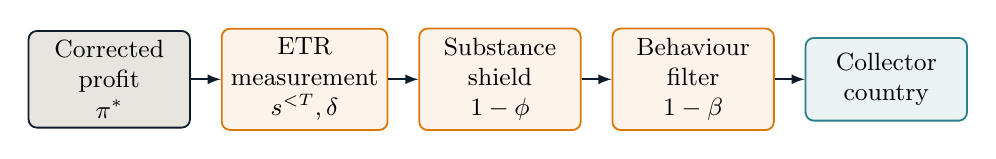
\begin{tikzpicture}[font=\small, node distance=0.42cm]
  \tikzset{
    stage/.style={draw=Navy, line width=0.65pt, rounded corners=3pt,
      fill=WarmGrey, minimum width=2.05cm, minimum height=1.05cm, align=center},
    filt/.style={draw=DkOrange, line width=0.65pt, rounded corners=3pt,
      fill=DkOrange!8, minimum width=2.05cm, minimum height=1.05cm, align=center},
    alloc/.style={draw=Teal, line width=0.65pt, rounded corners=3pt,
      fill=Teal!10, minimum width=2.05cm, minimum height=1.05cm, align=center},
    arr/.style={-latex, draw=Navy, line width=0.65pt}
  }
  \node[stage] (profit) {Corrected\\profit\\$\pi^{*}$};
  \node[filt, right=0.38cm of profit] (etr) {ETR\\measurement\\$s^{<T},\delta$};
  \node[filt, right=0.38cm of etr] (sub) {Substance\\shield\\$1-\phi$};
  \node[filt, right=0.38cm of sub] (beh) {Behaviour\\filter\\$1-\beta$};
  \node[alloc, right=0.38cm of beh] (col) {Collector\\country};
  \draw[arr] (profit) -- (etr);
  \draw[arr] (etr) -- (sub);
  \draw[arr] (sub) -- (beh);
  \draw[arr] (beh) -- (col);
\end{tikzpicture}
\end{center}

\vspace{0.45em}
\[
L_{p,j,t} =
\underbrace{s_{j,t}^{<T}\pi_{p,j,t}^{*}\bar{\delta}_{j,t}^{top}}_{\text{Stage 1: low-taxed base}}
\times
\underbrace{(1-\bar{\phi}_{p,j,t})}_{\text{Stage 2: unshielded part}}
\times
\underbrace{(1-\beta_{j,t})}_{\text{Stage 3: remaining profit}}
\]

\vspace{0.15em}
\small
\emphbx{Important distinction:} this slide defines the measured objects. The methodological slides explain how I estimate or vary them.
\note{Present this as the bridge between tax and statistics. Every tax detail is allowed into the talk only if it changes one of the pipeline variables.}
\end{frame}

\begin{frame}{Stage 1: identify low-taxed mass inside the average}
\begin{columns}[T]
\begin{column}{0.48\textwidth}
\begin{block}{Main comparison}
  \textbf{Jurisdiction-average ETR:} simple benchmark, but treats the whole cell as either below or above 15\%.\\[5pt]
  \textbf{Distributional or direct bracket:} estimates the profit mass below 15\% inside the cell.
\end{block}
\end{column}
\begin{column}{0.48\textwidth}
\begin{exampleblock}{Current source hierarchy}
  Direct Table IV where observed; Table I percentile fit where direct brackets are missing; early-year bracket-share transport where needed; average fallback only as last resort.
\end{exampleblock}
\end{column}
\end{columns}

\vspace{0.65em}
\begin{center}
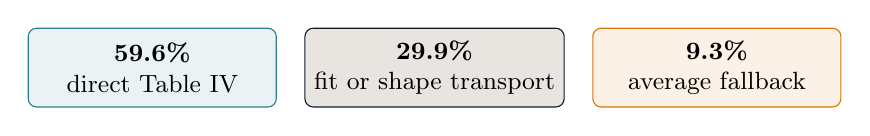
\begin{tikzpicture}[font=\small, node distance=0.35cm]
  \tikzset{
    stat/.style={draw=Navy, rounded corners=3pt, fill=WarmGrey,
      minimum width=3.15cm, minimum height=1.0cm, align=center},
    statb/.style={draw=Teal, rounded corners=3pt, fill=Teal!10,
      minimum width=3.15cm, minimum height=1.0cm, align=center},
    statc/.style={draw=DkOrange, rounded corners=3pt, fill=DkOrange!10,
      minimum width=3.15cm, minimum height=1.0cm, align=center}
  }
  \node[statb] (direct) {\textbf{59.6\%}\\direct Table IV};
  \node[stat, right=0.35cm of direct] (modelled) {\textbf{29.9\%}\\fit or shape transport};
  \node[statc, right=0.35cm of modelled] (fallback) {\textbf{9.3\%}\\average fallback};
\end{tikzpicture}
\end{center}

\vspace{0.1em}
\centering
\scriptsize
The core point is the ordering: use direct bracket evidence first, model the distribution only when needed.
\note{Keep this very simple. The audience only needs to understand that Stage 1 is not just theta divided by pi. The key decision is whether low-taxed mass is hidden inside an average.}
\end{frame}

\begin{frame}{Stage 2: substance changes the effective floor}
\begin{columns}[T]
\begin{column}{0.48\textwidth}
\begin{block}{Aggregate branch}
  CbCR supplies country-level payroll and tangible assets. This gives the baseline Substance-Based Income Exclusion (SBIE) shield:
  \[
  \text{SBIE}_{p,j,t}=\sigma_W W_{p,j,t}+\sigma_A A_{p,j,t}.
  \]
\end{block}
\end{column}
\begin{column}{0.48\textwidth}
\begin{exampleblock}{Sectoral branch}
  CbCR has no sector detail. FATS and EU KLEMS allocate country-level payroll, assets and profit across EU sectors, so I can test whether capital-intensive sectors face a lower effective floor under the Substance-Based Tax Incentive (SBTI) layer.
\end{exampleblock}
\end{column}
\end{columns}

\vspace{0.5em}
\begin{center}
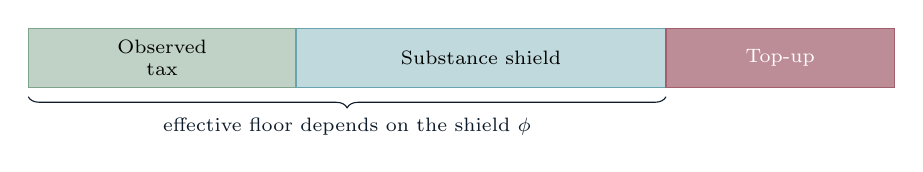
\begin{tikzpicture}[font=\small]
  \fill[ForestGreen!35, draw=ForestGreen!70] (0,0) rectangle (3.4,0.75);
  \fill[Teal!30, draw=Teal!70] (3.4,0) rectangle (8.1,0.75);
  \fill[Bordeaux!50, draw=Bordeaux!70] (8.1,0) rectangle (11,0.75);
  \node[font=\scriptsize, align=center] at (1.7,0.38) {Observed\\tax};
  \node[font=\scriptsize, align=center] at (5.75,0.38) {Substance shield};
  \node[font=\scriptsize, white] at (9.55,0.38) {Top-up};
  \draw[decorate, decoration={brace, mirror, amplitude=4pt}, Navy]
    (0,-0.12) -- node[below=4pt, font=\scriptsize]
    {effective floor depends on the shield $\phi$} (8.1,-0.12);
\end{tikzpicture}
\end{center}
\note{This is where the sectoral contribution enters. Be explicit that FATS is not a tax dataset. It is a sectoral allocation bridge used to study exposure and heterogeneity.}
\end{frame}

\section{Methodology}

\begin{frame}{Econometric method: estimate the behavioural filter}
\begin{center}
\footnotesize
$\log \pi_{p,j,t}^{*}
=
\beta_1\log A_{p,j,t}
+\beta_2\log \hat{W}_{p,j,t}
+f(\tau_{p,j,t})
+\boldsymbol{\beta}_x\mathbf{X}_{j,t}
+\alpha_{p,j}
+\gamma_t
+\varepsilon_{p,j,t}.$
\end{center}

\vspace{-0.05em}
\begin{center}
\scriptsize
\begin{tabular}{@{}L{3.2cm}L{4.2cm}L{4.0cm}@{}}
  \toprule
  \textbf{Choice} & \textbf{Baseline} & \textbf{Reason} \\
  \midrule
  Fixed effects & parent-affiliate pair and year & use within-pair tax variation, absorb persistent bilateral confounders \\
  Tax function & linear, quadratic and logarithmic & test whether low-rate response is sharply nonlinear \\
  Model selection & BIC ranking & avoid choosing the revenue answer by assumption \\
  Inference & two-way parent and affiliate clustering & allow correlated shocks by reporting and host jurisdiction \\
  \bottomrule
\end{tabular}
\end{center}

\vspace{0.05em}
\scriptsize
\emphbx{Estimated object:} a CbCR-cell semi-elasticity of reported profit, not a firm-level micro causal effect.
\note{This is the most important econometric slide. Say: the object is not a firm-level causal effect, it is a panel semi-elasticity for reported profit in CbCR cells.}
\end{frame}

\begin{frame}{Simulation method: 32 scenarios, one controlled design}
\begin{center}
\scriptsize
\begin{tabular}{@{}L{2.5cm}L{3.7cm}L{3.7cm}L{2.4cm}@{}}
  \toprule
  \textbf{Factor} & \textbf{Level 0} & \textbf{Level 1} & \textbf{Pipeline stage} \\
  \midrule
  ETR measurement & jurisdiction-average ETR benchmark & direct or distributional low-taxed mass & Stage 1 \\
  Substance specification & aggregate CbCR shield & sectoral FATS bridge plus SBTI overlay & Stage 2 \\
  SBIE rates & initial transition rates & long-run 5\% and 5\% rates & Stage 2 \\
  Implementation regime & universal IIR and UTPR collection & January 2026 Side-by-Side regime & Allocation \\
  Behaviour & mechanical no-response revenue & panel-estimated behavioural filter & Stage 3 \\
  \bottomrule
\end{tabular}
\end{center}

\vspace{0.55em}
\begin{block}{How to read the levels}
  Level 0 and Level 1 are coding labels for the factorial ANOVA. They are not ``low quality'' and ``high quality'', and they do not always mean lower or higher revenue.
\end{block}
\note{Make this explicit because the old low/high wording was confusing. The design is a controlled comparison of modelling choices, not a ranking of good and bad assumptions.}
\end{frame}

\section{Results}

\begin{frame}{Result 1: behavioural response is significant but moderate}
\begin{columns}[T]
\begin{column}{0.46\textwidth}
\begin{center}
\scriptsize
\begin{tabular}{@{}lrr@{}}
  \toprule
  Model & BIC rank & $\Delta$BIC \\
  \midrule
  Linear & 1 & 0.00 \\
  Logarithmic & 2 & 5.26 \\
  Quadratic & 3 & 7.56 \\
  \bottomrule
\end{tabular}
\end{center}

\vspace{0.3em}
\begin{block}{Preferred estimate}
  Linear ETR coefficient: $-1.506$, two-way clustered SE $0.273$, $p=1.6\times10^{-6}$.
\end{block}
\end{column}
\begin{column}{0.50\textwidth}
\begin{center}
\scriptsize
\begin{tabular}{@{}lrr@{}}
  \toprule
  Model and ETR & Semi-elasticity & Reallocation \\
  \midrule
  Linear, 5\% & 1.51 & 14.0\% \\
  Linear, 10\% & 1.51 & 7.3\% \\
  Quadratic, 5\% & 1.72 & 15.5\% \\
  Logarithmic, 5\% & 2.02 & 16.6\% \\
  \bottomrule
\end{tabular}
\end{center}

\vspace{0.3em}
\begin{alertblock}{Meaning}
  Behaviour lowers revenue, but the panel does not support the strongest claim that the low-ETR tail dominates the whole revenue answer.
\end{alertblock}
\end{column}
\end{columns}
\note{The clean message: I expected stronger nonlinearity, but the baseline evidence selects the linear model. This is a strength, not a problem, because it shows the thesis is not forcing the initial hypothesis.}
\end{frame}

\begin{frame}{Result 2: ETR measurement and SbS allocation explain the spread}
\begin{center}
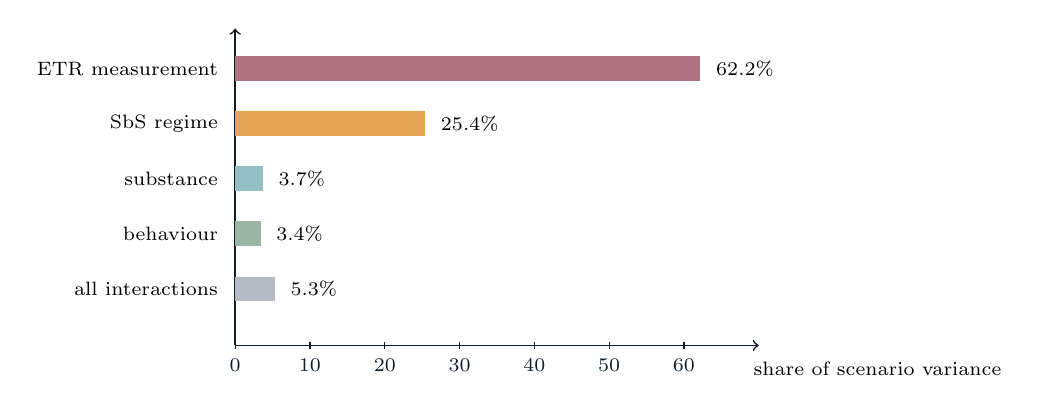
\begin{tikzpicture}[font=\small, xscale=0.095, yscale=0.70]
  \draw[->, Navy, line width=0.6pt] (0,0) -- (70,0);
  \draw[->, Navy, line width=0.6pt] (0,0) -- (0,5.75);
  \foreach \x/\lbl in {0/0,10/10,20/20,30/30,40/40,50/50,60/60} {
    \draw[Navy] (\x,0.07) -- (\x,-0.07) node[below, font=\scriptsize] {\lbl};
  }

  \fill[Bordeaux!62] (0,4.8) rectangle (62.2,5.25);
  \fill[DkOrange!68] (0,3.8) rectangle (25.4,4.25);
  \fill[Teal!50] (0,2.8) rectangle (3.7,3.25);
  \fill[ForestGreen!55] (0,1.8) rectangle (3.4,2.25);
  \fill[MidGrey!75] (0,0.8) rectangle (5.3,1.25);

  \node[font=\scriptsize, anchor=east] at (-1,5.02) {ETR measurement};
  \node[font=\scriptsize, anchor=east] at (-1,4.02) {SbS regime};
  \node[font=\scriptsize, anchor=east] at (-1,3.02) {substance};
  \node[font=\scriptsize, anchor=east] at (-1,2.02) {behaviour};
  \node[font=\scriptsize, anchor=east] at (-1,1.02) {all interactions};

  \node[font=\scriptsize, anchor=west] at (63.0,5.02) {62.2\%};
  \node[font=\scriptsize, anchor=west] at (26.2,4.02) {25.4\%};
  \node[font=\scriptsize, anchor=west] at (4.5,3.02) {3.7\%};
  \node[font=\scriptsize, anchor=west] at (4.2,2.02) {3.4\%};
  \node[font=\scriptsize, anchor=west] at (6.1,1.02) {5.3\%};
  \node[font=\scriptsize, anchor=west] at (68,-0.42) {share of scenario variance};
\end{tikzpicture}
\end{center}

\vspace{0.15em}
\small
\emphbx{Meaning:} disagreement across credible revenue estimates is mainly about Stage 1 measurement and legal allocation, not about the behavioural coefficient alone.
\note{This slide is the main result. Say that ETR measurement is an epistemic measurement problem; SbS is an institutional allocation problem. Both dominate the econometric behavioural main effect.}
\end{frame}

\begin{frame}{Result 3: revenue magnitudes confirm the ordering}
\begin{center}
\small
\begin{tabular}{@{}lrrr@{}}
  \toprule
  Factor change & Level 0 & Level 1 & Difference \\
  \midrule
  ETR measurement & 195.1 & 400.7 & +205.6 \\
  SbS regime & 356.5 & 239.2 & -117.3 \\
  Behavioural response & 321.4 & 274.3 & -47.1 \\
  Substance specification & 319.2 & 276.6 & -42.6 \\
  SBIE rate endpoint & 293.4 & 302.3 & +9.0 \\
  \bottomrule
\end{tabular}
\end{center}

\vspace{0.6em}
\begin{block}{Interpretation}
  Cumulative EU collector-country revenue over 2017 to 2022 ranges from \USD125.8 to 553.9 billion across the 32 scenarios. The table reports main effects averaged over all other factors.
\end{block}
\note{Connect the variance result to euros and dollars. The behavioural response is not small in money terms; it is smaller relative to measurement and allocation choices.}
\end{frame}

\begin{frame}{Result 4: Side-by-Side changes who collects}
\begin{columns}[T]
\begin{column}{0.47\textwidth}
\begin{block}{Mechanism}
  For qualifying US-parented groups, residual IIR and UTPR collection is set to zero. Domestic QDMTTs still collect where they exist.
\end{block}

\vspace{0.35em}
This changes \emph{who collects}, not the underlying amount of low-taxed profit.
\end{column}
\begin{column}{0.49\textwidth}
\begin{center}
\small
\begin{tabular}{@{}lrr@{}}
  \toprule
  Channel & Universal & SbS \\
  \midrule
  QDMTT & 201.4 & 201.4 \\
  IIR & 93.0 & 93.0 \\
  UTPR & 237.2 & 67.8 \\
  \midrule
  Total & 531.6 & 362.1 \\
  \bottomrule
\end{tabular}
\end{center}

\vspace{0.15em}
\centering
\scriptsize Preferred mechanical core, cumulative US\$ bn.
\end{column}
\end{columns}
\note{Do not get stuck in IIR and UTPR detail. The one point is that the legal channel can erase EU residual collection while leaving source-country QDMTTs untouched.}
\end{frame}

\begin{frame}{Result 5: sectoral SBTI exposure is concentrated}
\begin{columns}[T]
\begin{column}{0.52\textwidth}
\begin{center}
\scriptsize
\begin{tabular}{@{}lrrr@{}}
  \toprule
  Country & Before & After & Change \\
  \midrule
  EU27 weighted & 14.2 & 11.9 & -2.2 \\
  Netherlands & 14.5 & 13.6 & -0.9 \\
  Ireland & 14.7 & 13.7 & -1.0 \\
  Luxembourg & 14.2 & 13.7 & -0.5 \\
  Germany & 13.9 & 10.8 & -3.1 \\
  France & 13.8 & 10.3 & -3.5 \\
  \bottomrule
\end{tabular}

\vspace{0.2em}
\tiny Effective floor in percent; change in percentage points.
\end{center}
\end{column}
\begin{column}{0.44\textwidth}
\begin{exampleblock}{What it means}
  The SBTI overlay lowers the effective floor more in countries whose foreign-controlled sectors are more capital-intensive.
\end{exampleblock}

\vspace{0.35em}
\small
\emphbx{Caveat:} public data measure \emph{exposure capacity}, not actual safe-harbour elections or qualifying credit claims.
\end{column}
\end{columns}
\note{This is the sectoral part the old deck underplayed. Emphasise the caveat. The result is valuable because it shows heterogeneous exposure, not because it perfectly observes legal claims.}
\end{frame}

\begin{frame}{Current thesis position}
\begin{center}
\small
\begin{tabular}{@{}L{2.1cm}L{4.3cm}L{4.9cm}@{}}
  \toprule
  \textbf{Question} & \textbf{Current evidence} & \textbf{Implication} \\
  \midrule
  Behavioural shape & significant tax effect, BIC selects linear & H1 is weakened, not forced \\
  Measurement & ETR measurement explains 62.2\% of variance & H2 is strongly supported \\
  Interactions & all interactions explain 5.3\% & H3 is not supported at the 10\% threshold \\
  SbS allocation & preferred core falls from 531.6 to 362.1 & H4 is supported \\
  Sectoral SBTI & floor falls most in capital-intensive cells & H5 is supported with caveat \\
  \bottomrule
\end{tabular}
\end{center}

\vspace{0.5em}
\centering
\highlight{The result is becoming cleaner: the thesis explains why revenue estimates differ, not only what one preferred number is.}
\note{End the substantive talk here. This replaces the feedback slide. It tells the supervisors what has changed since the proposal and where the thesis now stands.}
\end{frame}

{
\setbeamercolor{background canvas}{bg=Navy}
\begin{frame}[plain]
  \vspace{1.5em}
  \begin{center}
    {\color{Ivory}\Large\bfseries Thank you}\\[1.2em]
    {\color{DkOrange}\rule{4cm}{2pt}}\\[1.2em]
    {\color{WarmGrey}\normalsize Measurement framework: define the tax base and channels.}\\[0.45em]
    {\color{LtOrange}\normalsize Methodology: estimate behaviour and decompose scenario variance.}\\[0.45em]
    {\color{WarmGrey}\normalsize Main result: measurement and allocation dominate current revenue uncertainty.}\\[1.2em]
    {\color{MidGrey}\small Maurits de Haan $\cdot$ m.c.p.dehaan@students.uu.nl}
  \end{center}
\end{frame}
}

\appendix

{
\setbeamercolor{background canvas}{bg=MidNavy}
\begin{frame}[plain]
  \vfill
  \centering
  {\color{Ivory}\LARGE\bfseries Backup slides}\\[0.6em]
  {\color{DkOrange}\rule{4cm}{2pt}}
  \vfill
\end{frame}
}

\begin{frame}{Backup: cross-validation of the ETR fit}
\begin{center}
\small
\begin{tabular}{@{}lr@{}}
  \toprule
  Statistic & Value \\
  \midrule
  Overlap affiliate-years & 239 \\
  Low-taxed share, median gap & 0.117 \\
  Low-taxed share, mean absolute error & 0.293 \\
  Spearman correlation & 0.464 \\
  Calibration slope & 0.68 \\
  Calibration $R^2$ & 0.201 \\
  Wilcoxon $p$-value & $5.8\times10^{-10}$ \\
  \bottomrule
\end{tabular}
\end{center}

\vspace{0.6em}
\begin{alertblock}{Implication}
  The public percentile fit is informative but imperfect. This supports the thesis decision to put ETR measurement at the centre of the uncertainty decomposition.
\end{alertblock}
\end{frame}

\begin{frame}{Backup: selected country scenario spreads}
\begin{center}
\small
\begin{tabular}{@{}lrrr@{}}
  \toprule
  Country & Minimum & Maximum & Spread \\
  \midrule
  Netherlands & 44.0 & 129.8 & 85.9 \\
  Germany & 11.2 & 105.9 & 94.7 \\
  France & 5.2 & 55.7 & 50.4 \\
  Ireland & 20.0 & 52.7 & 32.7 \\
  Luxembourg & 11.0 & 49.4 & 38.4 \\
  \bottomrule
\end{tabular}
\end{center}

\vspace{0.5em}
\centering
\scriptsize Cumulative collector-country revenue over 2017 to 2022, US\$ bn.
\end{frame}

\begin{frame}{Backup: SBTI sectoral exposure}
\begin{center}
\small
\begin{tabular}{@{}lrrr@{}}
  \toprule
  Country & Floor before SBTI & Floor after SBTI & Change \\
  \midrule
  EU27 weighted & 14.2 & 11.9 & -2.2 \\
  Netherlands & 14.5 & 13.6 & -0.9 \\
  Ireland & 14.7 & 13.7 & -1.0 \\
  Germany & 13.9 & 10.8 & -3.1 \\
  France & 13.8 & 10.3 & -3.5 \\
  \bottomrule
\end{tabular}
\end{center}

\vspace{0.6em}
\begin{block}{Caveat}
  Public data do not observe actual qualifying tax incentive claims. The sectoral branch is therefore best interpreted as exposure to SBTI capacity, not as a point forecast of elections.
\end{block}
\end{frame}

\begin{frame}{Backup: why pair fixed effects matter}
\begin{center}
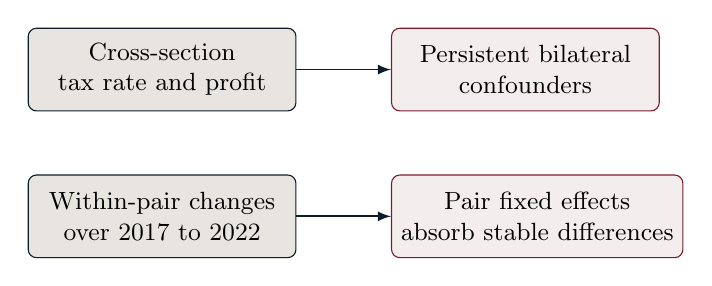
\begin{tikzpicture}[font=\small, node distance=0.6cm]
  \tikzset{
    obs/.style={draw=Navy, rounded corners=3pt, fill=WarmGrey,
      minimum width=3.4cm, minimum height=1.05cm, align=center},
    fe/.style={draw=Bordeaux, rounded corners=3pt, fill=Bordeaux!8,
      minimum width=3.4cm, minimum height=1.05cm, align=center},
    arr/.style={-latex, draw=Navy, line width=0.65pt}
  }
  \node[obs] (cross) {Cross-section\\tax rate and profit};
  \node[fe, right=1.2cm of cross] (conf) {Persistent bilateral\\confounders};
  \node[obs, below=0.8cm of cross] (panel) {Within-pair changes\\over 2017 to 2022};
  \node[fe, right=1.2cm of panel] (clean) {Pair fixed effects\\absorb stable differences};
  \draw[arr] (cross) -- (conf);
  \draw[arr] (panel) -- (clean);
\end{tikzpicture}
\end{center}

\vspace{0.7em}
\begin{block}{Interpretation}
  A cross-section risks comparing structurally different country pairs. The panel asks whether the same parent-affiliate pair reports different profit when its effective tax rate changes.
\end{block}
\end{frame}

\end{document}
